
\chapter{Estudio teórico}
\label{cha:estudio-teorico}

Aquí se explicará el estado de arte actual \ldots

\begin{figure}[!h]
\centering
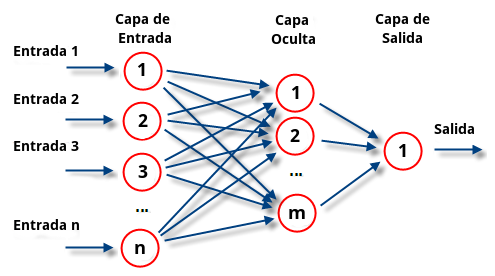
\includegraphics[width=0.8\textwidth]{img/rnn.png}
\caption{\label{fig:rnn}Red neuronal \ldots}
\end{figure}
La figura \ref{fig:rnn} muestra \ldots

\section{Introducción}
\label{sec:intro-sota}

\section{Estado del arte}
\label{sec:sota}

\section{Técnicas utilizadas}
\label{sec:tecnicas-utilizadas}

\subsection{YOLOv4 + Tensorflow 2}
\label{sec:tecnicas-utilizadas1}

\subsection{DeepSort}
\label{sec:tecnicas-utilizadas2}

\section{Conclusiones}
\label{sec:conclu-sota}